\documentclass{beamer}
\usepackage{beamerthemesplit} 
\usepackage{hyperref}

\title{Les tests de logiciel}
\author {\href{mailto:sofien.benharchache@etud.univ-montp2.fr}{Sofien Benharchache} \and \href{mailto:stella.zevio@etud.univ-montp2.fr}{Stella Zevio}}
\institute{Universit\'{e} Montpellier II}
\date{16 octobre 2014}

\begin{document}

\frame{\titlepage}

\frame{
	\frametitle{Sommaire}
	\begin{enumerate}
		\item Introduction	
		\item M\'{e}thodes de v\'{e}rification et validation
		\item Principes de base et mauvaises pratiques
		\item Diff\'{e}rentes classifications de tests
		\item Frameworks et outils de test
		\item Conclusion
	\end{enumerate}
}

\frame{
	\frametitle{Sommaire - Introduction}
	\begin{enumerate}
		\item Introduction
			\begin{enumerate}
				\item Qu'est-ce qu'un logiciel ? 
				\item Qu'est-ce qu'un test de logiciel ? 
				\item Qu'est-ce qu'un bug ?
				\item Pourquoi tester un logiciel ?
			\end{enumerate}	
	\end{enumerate}
}

\begin{frame}
	\frametitle{Qu'est-ce qu'un logiciel ?}
	\framesubtitle{}
 
 	\begin{itemize}
		\item Des documents de gestion de projet
		\item La sp\'{e}cification
		\item La conception 
		\item Le code source
		\item L'ex\'{e}cutable
	\end{itemize}
\end{frame}

\begin{frame}
	\frametitle{Qu'est-ce qu'un test de logiciel ?}
	\framesubtitle{}
		
			\begin{itemize}
				\item Propri\'{e}t\'{e}s
				\item R\'{e}sultat
				\begin{itemize}
					\item Validation dynamique
				\end{itemize}
			\end{itemize}	
			\tiny{norme IEEE-STD729, 1983}
		
\end{frame}

\begin{frame}
	\frametitle{Qu'est-ce qu'un bug ?}
	
	Erreur $\rightarrow$ D\'{e}faut $\rightarrow$ Anomalie
\end{frame}

\begin{frame}
	\frametitle{Pourquoi tester un logiciel ?}
	\framesubtitle{\'{E}viter les bugs}
		\begin{figure}
			\centering
			\caption{Sonde Mariner 1, 1962}
			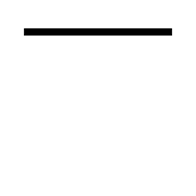
\includegraphics[scale=0.20]{img/mariner}
		\end{figure}
\end{frame}

\begin{frame}
	\frametitle{Pourquoi tester un logiciel ?}
	\framesubtitle{\'{E}viter les bugs}
		\begin{figure}
			\centering
			\caption{Ariane 5 vol 501, 1996}
			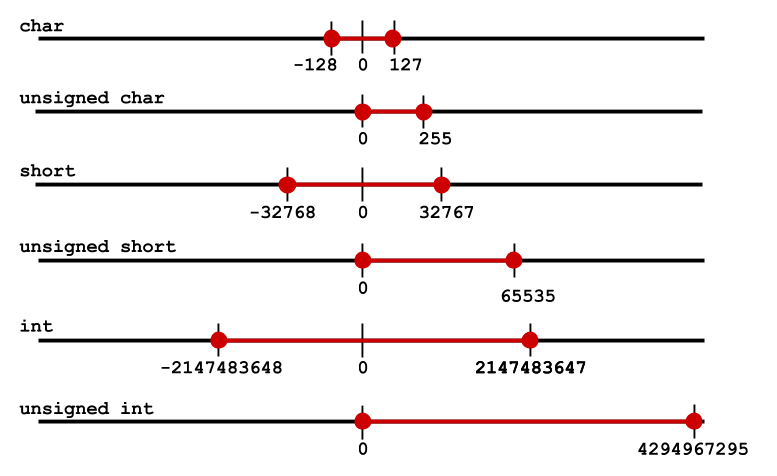
\includegraphics[scale=0.25]{img/ariane}
		\end{figure}
\end{frame}

\begin{frame}
	\frametitle{Pourquoi tester un logiciel ?}
	\framesubtitle{\'{E}viter les bugs}
		\begin{figure}
			\centering
			\caption{Therac-25, 1985-1987}
			
\includegraphics[scale=0.07]{img/therac}
		\end{figure}
\end{frame}

\begin{frame}
	\frametitle{Pourquoi tester un logiciel ?}
	\framesubtitle{R\'{e}duire les co\^{u}ts}
		\begin{figure}
			\centering
			\caption{Applied Software Measurement, Capers Jones, 1996}
			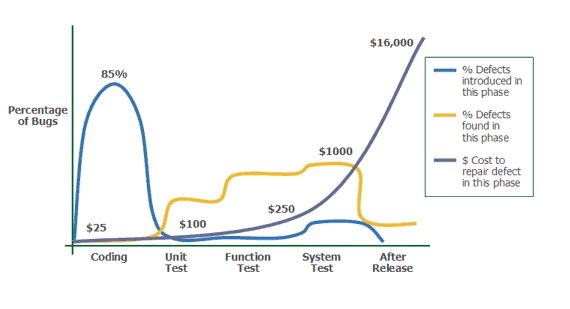
\includegraphics[scale=0.50]{img/defect}
		\end{figure}
\end{frame}

\begin{frame}
	\frametitle{Pourquoi tester un logiciel ?}
	\framesubtitle{R\'{e}duire les co\^{u}ts}
		\begin{itemize}
			\item 30-50\% des co\^{u}ts de d\'{e}veloppement
			\item 1/3 dans le planning
		\end{itemize}	
\end{frame}

\begin{frame}
	\frametitle{Pourquoi tester un logiciel ?}
	\framesubtitle{Assurer la qualit\'{e}}
		\begin{itemize}
			\item Capacit\'{e} fonctionnelle
			\item Facilit\'{e} d'utilisation
			\item Fiabilit\'{e}
			\item Performance
			\item Maintenabilit\'{e}
			\item Portabilit\'{e}
		\end{itemize}
\end{frame}

\frame{
	\frametitle{Sommaire - M\'{e}thodes de v\'{e}rification et validation}
	\begin{enumerate}
		\item Introduction
		\item M\'{e}thodes de v\'{e}rification et validation
			\begin{enumerate}
				\item M\'{e}thodes de v\'{e}rification et validation
				\item Comparaison des m\'{e}thodes
			\end{enumerate}	
	\end{enumerate}
}

\begin{frame}
	\frametitle{M\'{e}thodes de v\'{e}rification et validation}
	\framesubtitle{V\'{e}rification et validation}
		\begin{description}
		\item[V\'{e}rification] \textit{"are we building the product right ?"} 
			\begin{itemize}
				\item Preuve formelle, model-checking
			\end{itemize}	
			\bigskip			
		\item[Validation] \textit{"are we building the right product ?"} 
			\begin{itemize}
				\item Test
			\end{itemize}
		\end{description}
\end{frame}


\begin{frame}
	\frametitle{Comparaison des m\'{e}thodes de v\'{e}rification et validation}
	\framesubtitle{}
	
		Preuve formelle, model-checking
		\begin{itemize}
			\item Exhaustifs
			\item Mise en \oe{}uvre difficile
			\item Limitations par rapport \`{a} la taille du syst\`{e}me
			\item Distance entre le mod\`{e}le et la r\'{e}alit\'{e}
		\end{itemize}
		
		\bigskip
		
		Test
		\begin{itemize}
			\item N\'{e}cessaire mais pas suffisant
			\item N\'{e}cessite une ex\'{e}cution r\'{e}elle du syst\`{e}me
			\item Ne garantit pas l'absence d'erreur
		\end{itemize}
\end{frame}	

\frame{
	\frametitle{Sommaire - Principes de base et mauvaises pratiques}
	\begin{enumerate}
		\item Introduction	
		\item M\'{e}thodes de v\'{e}rification et validation
		\item Principes de base, bonnes et mauvaises pratiques
			\begin{itemize}
				\item Mauvaises pratiques
				\item Bonnes pratiques
				\item Principes de base
			\end{itemize}
	\end{enumerate}
}

\begin{frame}
	\frametitle{Principes de base, bonnes et mauvaises pratiques}
	\framesubtitle{Mauvaises pratiques}
		
	Tenter d'isoler un bug \`{a} l'aide d'appels d'affichage.

\end{frame}

\begin{frame}
	\frametitle{Principes de base, bonnes et mauvaises pratiques}
	\framesubtitle{Bonnes pratiques}
		\begin{enumerate}
			\item Objectifs
			\item Donn\'{e}es de test, r\'{e}sultats attendus
			\item Ex\'{e}cution, collecte des r\'{e}sultats
			\item Comparaison, \'{e}tablissement d'un verdict
		\end{enumerate}
\end{frame}	
	
\begin{frame}
	\frametitle{Principes de base et mauvaises pratiques}
	\framesubtitle{Principes de base}
	
		\begin{enumerate}
			\item Ne pas tester ses propres programmes
			\item Chercher les erreurs
			\item D\'{e}finir les r\'{e}sultats  attendus avant d'ex\'{e}cuter un test
			\item Inspecter minutieusement les traces
			\item Prendre en compte les entr\'{e}es invalides ou incoh\'{e}rentes
			\item V\'{e}rifier que le programme n'en fait pas plus que sa sp\'{e}cification
		\end{enumerate}
\end{frame}

\frame{
	\frametitle{Sommaire - Diff\'{e}rentes classifications de tests}
	\begin{enumerate}
		\item Introduction	
		\item M\'{e}thodes de v\'{e}rification et validation
		\item Principes de base et mauvaises pratiques
		\item Diff\'{e}rentes classifications de tests
			\begin{itemize}
				\item Classification selon le niveau
				\begin{itemize}
					\item Cycle de d\'{e}veloppement en V d'un logiciel
				\end{itemize}
				\item Classification selon le niveau d'accessibilit\'{e}
				\begin{itemize}
					\item Bo\^{i}te noire
					\item Bo\^{i}te blanche
				\end{itemize}	
				\item Classification selon les caract\'{e}ristiques
			\end{itemize}
	\end{enumerate}
}

\begin{frame}
	\frametitle{Classifications de tests}
	\framesubtitle{Classification selon le niveau}
		\begin{itemize}
			\item Test unitaire
			\item Test d'int\'{e}gration
			\item Test syst\`{e}me
			\item Test d'acceptation ou recette
		\end{itemize}
		
		\tiny{Comit\'{e} fran\c{c}ais du test logiciel}
\end{frame}



\begin{frame}
	\frametitle{Classification selon le niveau}
	\framesubtitle{Cycle de d\'{e}veloppement en V}
	
		\begin{figure}
			\centering
			\caption{Cycle de d\'{e}veloppement en V d'un logiciel}
			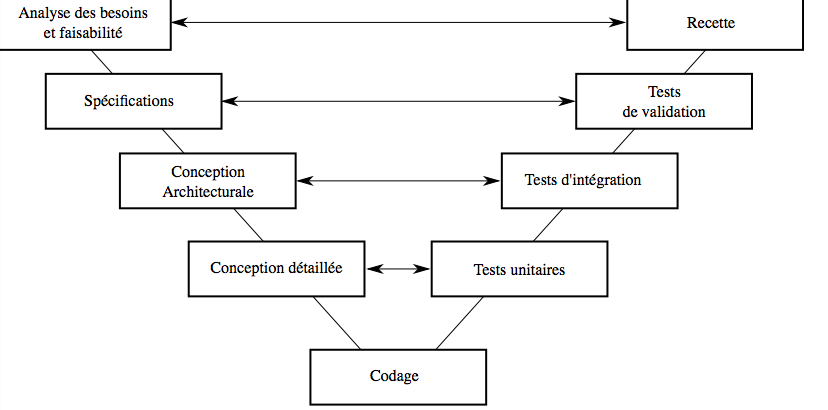
\includegraphics[scale=0.39]{img/niveau}
		\end{figure}	
\end{frame}

\begin{frame}
	\frametitle{Classification de tests}
	\framesubtitle{Classification selon le niveau d'accessibilit\'{e}}
		\begin{itemize}
			\item Bo\^{i}te noire
			\item Bo\^{i}te blanche
		\end{itemize}
\end{frame}

\begin{frame}
	\frametitle{Classification selon le niveau d'accessibilit\'{e}}
	\framesubtitle{Bo\^{i}te noire}
	
		\begin{figure}
			\centering
			\caption{Bo\^{i}te noire}
			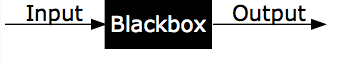
\includegraphics[scale=0.5]{img/boitenoire}
		\end{figure}	
\end{frame}

\begin{frame}
	\frametitle{Classification selon le niveau d'accessibilit\'{e}}
	\framesubtitle{Bo\^{i}te blanche}
		\par Code source d\'{e}j\`{a} \'{e}crit.			
\end{frame}

\begin{frame}
	\frametitle{Classification de tests}
	\framesubtitle{Classification selon les caract\'{e}ristiques}
	
		\begin{itemize}
			\item Performance
			\item Robustesse
			\item Vuln\'{e}rabilit\'{e}
			\item Non r\'{e}gression
		\end{itemize}
		\tiny{Liste non exhaustive}
\end{frame}

\frame{
	\frametitle{Sommaire - Frameworks et outils de test}
	\begin{enumerate}
		\item Introduction	
		\item M\'{e}thodes de v\'{e}rification et validation
		\item Principes de base et mauvaises pratiques
		\item Diff\'{e}rentes classifications de tests
		\item Frameworks et outils de test
	\end{enumerate}
}

\begin{frame}
	\frametitle{Frameworks et outils de test}
	\framesubtitle{}
	
		\begin{itemize}
			\item Frameworks (xUnit)
			\item Objets de type mock (programmation orient\'{e}e objet)
			\item JMeter
			\item SoapUI...
			\item Outils de couverture de code (TestWellCTC++, Emma, Xdebug...)
		\end{itemize}
		
\end{frame}

\frame{
	\frametitle{Sommaire - Conclusion}
	\begin{enumerate}
		\item Introduction	
		\item M\'{e}thodes de v\'{e}rification et validation
		\item Principes de base et mauvaises pratiques
		\item Diff\'{e}rentes classifications de tests
		\item Frameworks et outils de test
		\item Conclusion
	\end{enumerate}
}

\begin{frame}
	\frametitle{Conclusion}
	\framesubtitle{Tester, c'est tr\`{e}s important}
	
		Tester, c'est :
		\begin{itemize}
			\item Une activit\'{e} \`{a} part enti\`{e}re
			\item Avoir une vision globale d'un logiciel \`{a} toutes les \'{e}tapes de son d\'{e}veloppement
		\end{itemize}
		
		\bigskip
		
		Tester, \c{c}a doit \^{e}tre :
		\begin{itemize}	
			\item Une activit\'{e} rigoureuse
			\item De plus en plus automatique
		\end{itemize}
\end{frame}

\begin{frame}
	\frametitle{Conclusion}
	\framesubtitle{Tester, c'est tr\`{e}s important}
	
	\textbf{Testez vos programmes !}
	
\end{frame}		

\end{document}
